\documentclass[a4paper,11pt,polish]{memoir}
% acelnosxz
% ����󶼿
% ��ʣ�Ӧ��
\usepackage[cp1250]{inputenc}
\usepackage[T1]{fontenc}
\usepackage{pslatex}
\usepackage[polish]{babel}
\usepackage{tabularx}
\usepackage{multicol}
\usepackage{color,colortbl}
\usepackage{calc,soul,fourier}
\usepackage{setspace}
\usepackage{indentfirst}
\usepackage{type1cm,eso-pic}
\usepackage{ifpdf}
\usepackage{amsmath}  
\usepackage{listings}
%\usepackage[nottoc]{tocbibind}
%\usepackage[titles]{tocloft}
%\usepackage{natbib}
\usepackage[sectionbib]{chapterbib}
\makeatletter
\renewcommand{\@memb@bsec}{\section*{\bibname}\prebibhook}
\makeatother

\usepackage{makeidx} \makeindex 
\ifpdf
 \usepackage[pdftex,bookmarks,breaklinks]{hyperref}
 \usepackage[pdftex]{graphicx}
 \DeclareGraphicsExtensions{.pdf,.jpg,.mps,.png}
 \pdfcompresslevel=9
\else
 \usepackage{graphicx}
 \DeclareGraphicsExtensions{.eps,.ps,.jpg,.mps,.png}
\fi

\makeatletter
\AddToShipoutPicture{%
  \setlength{\unitlength}{1mm}
  \put(18,29.5){\line(-1,0){10}}%
  \put(21,26.5){\line(0,-1){10}}%
  \put(192,29.5){\line(1,0){10}}%
  \put(189,26.5){\line(0,-1){10}}%
  \put(18,267.5){\line(-1,0){10}}%
  \put(21,270.5){\line(0,1){10}}%
  \put(192,267.5){\line(1,0){10}}%
  \put(189,270.5){\line(0,1){10}}%
}
\makeatother

%%%%%%%%%%%%%%%%%%%%%%%%%%%%%%%%%%%%%%%%%%%%%%%%%%%%%%%%%%%%%%%%%%%%%%%%%%%%%%%%%%%%%%%%%%%%%%%%%%%%%
%%    Ustawienia strony + definicje pomocnicze                                                     %%
%%%%%%%%%%%%%%%%%%%%%%%%%%%%%%%%%%%%%%%%%%%%%%%%%%%%%%%%%%%%%%%%%%%%%%%%%%%%%%%%%%%%%%%%%%%%%%%%%%%%%
%\setlength{\headsep}{0pt} \setlength{\headheight}{0pt}
\setlength{\hoffset}{0mm} %%a4
\setlength{\voffset}{0mm} %-14mm %%a4
\setlength{\footskip}{23pt} % 23pt ~= 8mm
\setlength{\topmargin}{11mm}%{7.65mm} %28pt -2.5mm
\setlength{\oddsidemargin}{11.85mm}
\setlength{\evensidemargin}{11.85mm}

\setlength{\textwidth}{135.5mm}
\setlength{\textheight}{203.6mm}

\setlength{\parindent}{18pt}
\setlength{\parskip}{0pt} %{1ex plus 0.5ex minus 0.2ex}

\setlength{\extrarowheight}{2pt}

\sloppy  % wyr�wnanie z dw�ch stron
\renewcommand{\topfraction}{1.0}
\renewcommand{\bottomfraction}{1.0}
\renewcommand{\textfraction}{0.0}

%\widowpenalty=10000 % ostatni wiersz akapitu nie zostanie przeniesiony na nast�pn� stron� 
%\clubpenalty=10000 % pierwszy wiersz akapitu nie b�dzie ko�czy� strony (nie u�ywam tego ustawienia)
%\tolerance = 500 \pretolerance = 900 %% sk�ad z wi�ksz� `tolerancj�' (mo�na te warto�ci zwi�kszy� bardziej)
%\hbadness= 1450 %% zmniejsza licz� wy�wietlanych ostrze�e� (mo�na zwi�kszy�, ale bez przesady)
%\hfuzz = 1.5pt %% tekst mo�e stercze� ma marginesie na 1,5pt (ok. 0,5mm)

%\setlength{\floatsep}{12pt}
%\setlength{\textfloatsep}{12pt}
%\setlength{\intextsep}{12pt}
%\setlength{\arrayrulewidth}{0.5pt}

\makeatletter
\renewenvironment{itemize}{
  \begin{list}{  
  \csname labelitem\romannumeral\the\@listdepth\endcsname}{
    \setlength{\leftmargin}{1em}
	\setlength{\topsep}{6pt}%
	\setlength{\partopsep}{0pt}%
	\setlength{\parskip}{0pt}%
	\setlength{\parsep}{0pt}%
	\setlength{\itemsep}{0pt}}
}{
  \end{list}
}
\renewenvironment{quote}{
  \begin{list}{}{}
	 \item[]}
	 {\unskip\end{list}}
\makeatother

\makeatletter
\newskip\@hlskip
%\@hlskip=.5\baselineskip \@plus 1mm \@minus .5mm
\@hlskip=6pt

\newdimen\verbatimleftmargin
  \verbatimleftmargin\z@
\newdimen\verbatimbaselineskip
  \verbatimbaselineskip\baselineskip
\def\verbatimsize{\normalsize}

\def\@verbatim{%
 \topsep\@hlskip
 \partopsep\z@\parsep\z@\itemsep\z@
 \trivlist \item\relax
  \if@minipage\else
   \vskip\baselineskip
   \vskip-\verbatimbaselineskip
%  \vskip\parskip
  \fi
  \leftskip\@totalleftmargin
  \if@minipage\else
   \advance \leftskip by \verbatimleftmargin
  \fi
  \rightskip\z@skip
  \parindent\z@\parfillskip\@flushglue\parskip\z@skip
  \@@par
  \@tempswafalse
  \def\par{%
    \if@tempswa
      \leavevmode \null \@@par\penalty\interlinepenalty
    \else
      \@tempswatrue
      \ifhmode\@@par\penalty\interlinepenalty\fi
    \fi}%
  \let\do\@makeother \dospecials
  \obeylines 
   \verbatimsize \baselineskip\verbatimbaselineskip
   \verbatim@font \@noligs
  \everypar \expandafter{\the\everypar \unpenalty}%
}

\makeatother

\definecolor{nicered}{rgb}{.647,.129,.149}
\newcommand{\autorzy}{}

\makeatletter
\newlength\dlf@normtxtw
\setlength\dlf@normtxtw{\textwidth}
\def\myhelvetfont{\def\sfdefault{mdput}}
\newsavebox{\feline@chapter}
\newcommand\feline@chapter@marker[1][4cm]{%
\sbox\feline@chapter{%
\resizebox{!}{#1}{\fboxsep=1pt%
\colorbox{nicered}{\color{white}\bfseries\sffamily\thechapter}%
}}%
\rotatebox{90}{%
\resizebox{%
\heightof{\usebox{\feline@chapter}}+\depthof{\usebox{\feline@chapter}}}%
{!}{\scshape\so\@chapapp}}\quad%
\raisebox{\depthof{\usebox{\feline@chapter}}}{\usebox{\feline@chapter}}%
}
\newcommand\feline@chm[1][4cm]{%
\sbox\feline@chapter{\feline@chapter@marker[#1]}%
\makebox[0pt][l]{% aka \rlap
\makebox[1cm][r]{\usebox\feline@chapter}%
}}
\makechapterstyle{daleif1}{
\renewcommand\chapnamefont{\normalfont\Large\scshape\raggedleft\so}
\renewcommand\chaptitlefont{\normalfont\huge\bfseries\scshape\color{nicered}}
\renewcommand\chapternamenum{}
\renewcommand\printchaptername{}
\renewcommand\printchapternum{\null\hfill\feline@chm[2.5cm]\par}
\renewcommand\afterchapternum{\par\vskip\midchapskip}
\renewcommand\printchaptertitle[1]{\chaptitlefont\raggedleft ##1\\  \makebox[\textwidth - (1cm + \widthof{\Huge \thechapter.})][r]{\Large \itshape \autorzy}\par}
}

%definicja nag��wk�w
\renewcommand{\chaptermark}[1]{\markboth{\ifnum \c@secnumdepth >\m@ne
      \thechapter \ \fi #1}{}} 
\renewcommand{\sectionmark}[1]{\markright{\thesection \ #1}{}} 
\setcounter{secnumdepth}{3}
%definicja g��boko�ci numerowania sekcji
\maxsecnumdepth{subsection}

% z jakiego� powodu czcionki s� mniejsze o jeden punkt ni� wynika�oby to z poni�szych ustawie�
\renewcommand{\bfdefault}{b}
\renewcommand{\normalsize}{\fontsize{11pt}{12.5pt}\selectfont}
\newcommand{\smallp}{\fontsize{9.5pt}{11.5pt}\selectfont}
\makeatother

%%% Strona tytu�owa
\newcommand*{\titleTH}{\begingroup% T&H Typography
\raggedleft
\vspace*{4cm}
{\bfseries Kolekcja prac}\\[\baselineskip]
{\textcolor{nicered}{\Huge 	KOMPUTEROWE}}\\[\baselineskip]
{\textcolor{nicered}{\Huge 	PRZETWARZANIE}}\\[\baselineskip]
{\textcolor{nicered}{\Huge 	WIEDZY}}\\[\baselineskip]
\vfill
{\Large Politechnika Wroc�awska, 2011}\par
\vspace*{3\baselineskip}
\endgroup}

\begin{document}
\thispagestyle{empty} \titleTH \cleardoublepage
\tableofcontents*
\thispagestyle{empty} \cleardoublepage

\chapterstyle{daleif1}
\bibliographystyle{myaplike}
\renewcommand{\autorzy}{P. Batog, M. Pichliński}
\chapter[Budowa modeli informacyjnych i ich profilowanie]
        [Budowa modeli informacyjnych i ich profilowanie]
        {Budowa modeli informacyjnych i ich profilowanie}

\section{Wstęp}
Rozwój komputerów i sprzętu elektronicznego oraz Internetu sprzyja zwiększaniu
ilości informacji oraz daje coraz to łatwiejszy do niej dostęp. W roku 2003
za pomocą wyszukiwarek internetowych (tzw. powierzchniowy Internet)
było dostępne 167 terabajtów danych (w porównaniu do 2000 roku jest ich
trzykrotnie więcej) \cite{HowMuchInformation}.
IBM w 2006 roku stwierdziło, że w 2010 ilość przechowywanej elektronicznej
informacji będzie zwiększała się dwukrotnie w przeciągu 11 godzin 
(nie koniecznie w samej sieci) \cite{ToxicTerabyte}.

Dodatkowo ,,powierzchnia'' Internetu to wierzchołek góry lodowej, ponieważ
ukryty (głęboki) Internet, czyli taki którego dane nie są dostępne 
bezpośrednio przez hiperlinki (np. wewnętrzne bazy danych) szacuje się na 500
krotnie większy niż to co na codzień można otrzymać dzięki Google 
\cite{DeepWeb}. Taka zatrważająca ilość informacji powoduje takie szkody jak: 
utrudnienie uzyskania potrzebnych danych, problemy z powstrzymaniem
wzrastającego chaosu informacyjnego, spowolnienie dostępu do danych z powodu
obciążenia powstałego w wyniku przeszukiwania zasobów \cite{ToxicTerabyte}.
Powyższe problemy wynikające z nadmiaru zasobów wiedzy, próbuje się rozwiązać 
za pomocą modeli informacyjnych. 

W niniejszej pracy zostanie przedstawione ontologiczne podejście w zagadnieniu budowy modelu informacji, na przykładzie tworzenia tezaurusa. 

\section{Czym są modele informacyjne?}
Modele informacyjne są to sposoby reprezentacji zasobów wiedzy, takich jak:
koncepty, relacje, ograniczenia, zasady, operacje. Polegają one na nadaniu
danym znaczenia semantycznego \cite{Tina}. Dzięki modelom informacyjnym,
wiedza, która jest w nich przechowywana, nabiera elastyczności pozwalającej 
na dzielenie jej pomiędzy różnymi aplikacjami, łatwiejsze wyszukiwanie
pożądanych informacji oraz dostosowanie do potrzeb użytkownika 
\cite{GilbaneReport}.


Warto wspomnieć o różnicy pomiędzy modelami informacyjnymi a modelami danych,
które mogą być mylnie utożsamiane ze sobą. Celem tych pierwszych jest 
zarządzanie modelami na poziomie ideowym oraz przedstawienie relacji pomiędzy
nimi, niezależnie od konkretnych implementacji bądź protokołów transmisji
danych. Model informacyjny jest narzędziem przeznaczonym dla projektantów.
Natomiast modele danych odnoszą się niższemu poziomowi abstrakcji, zawierają
więcej szczegółów, są one już konkretną implementacją modeli informacyjnych 
\cite{RFC3444}.



\section{Ontologia jako model informacji}
Celem stworzenia modelu informacji jest nadanie jej wyższego stopienia organizacji. Uporządkowanie ma zaś umożliwić łatwiejsze przetwarzanie informacji i wyciągania na ich podstawie określonych wniosków. Innymi słowy jest to dodanie abstrakcji umożliwiającej przechodzenie od informacji w kierunku do wiedzy. Budowa modelu informacji jest zagadnieniem z natury heurystycznym. Nie istnieją bowiem ogólne prawa, według których proces budowy takiego modelu miałby zostać przeprowadzony. 

Budowa modelu ściśle wiąże się z dziedziną i problemem, którego ma być rozwiązaniem. W dzisiejszych czasach dostępnych jest mnóstwo odpowiednich metod i technik. Co więcej poszczególne organizacje modyfikują ogólnie znane metody bazując na doświadczeniach w konkretnych zagadnieniach i technikach. Taka sytuacje bywa nazywana w literaturze ,,dżunglą metodologiczną'' \cite{Verhoef}. W niniejszej pracy skupiono się na podejściu ontologicznym.

\subsection{Ontologia}
Ontologia, jest reprezentacją dystrybuowanej konceptualizacji określonej domeny\footnote{Hodge}. Mówiąc prościej, jest budową wspólnej warstwy pojęciowej, rozwinięciem konceptualizacji poprzez dodanie relacji pomiędzy poszczególnymi podmiotami. Obydwa pojęcia mają swoje korzenie w naukach filozoficznych.
\begin{itemize}
   \item Konceptualizacja - próba określenia ścisłych pojęć, (usunięcie wieloznaczności) niezbędnych do opisu jednoznacznie rozumianego procesu z określonej dziedziny.
	\item Ontologia - (od greckich $o \nu \tau o$ - byt i $\iota o\gamma o\varsigma$ - nauka ) najogólniejsza nauka rozważająca pojęcie bytu, do XVII w utożsamiana z metafizyką. Jej początków można szukać u Arystotelesa. Dziedzina metafizyki, związana z badaniem, wyjaśnianiem natury, kluczowych właściwości oraz relacji rządzących wszelakimi bytami bądź głównych zasad i przyczyn bytu \footnote{Webster}.
\end{itemize}  

W praktyce technologii informacyjnej poprzez ontologię rozumie się jako  świadomą, formalną 
specyfikację konceptów (pojęć) w danej dziedzinie i relacji pomiędzy nimi. Ontologia łączy ze sobą nie tylko wyrażone w niej pojęcia, ale również wiedzę, która może być na jej podstawie wywnioskowana. Jako sposób reprezentacji zintegrowanego  modelu wiedzy dziedziny oraz jako instrument badawczy treści informacji tekstowej razem z innymi technologiami informatycznymi jest obecnie jednym z kluczowych elementów 
rozwijającej się idei społeczeństwa informacyjnego. Dowodem na to jest dynamiczny rozwój internetu trzeciej generacji \footnote{Semantic Web, Web 3.0 - http://www.slideshare.net/skruk/sie-semantyczna-w-teorii-i-praktyce}. 
 
\section{Tezaurus}
Tezaurus w ogólnym rozumieniu stanowi słownik terminów bliskoznacznych. Słowo pochodzi z greckiego $\Theta \eta \sigma \alpha \upsilon \rho o \varsigma$, gdzie oznaczało zbiór rzeczy o wielkiej wartości (magazyn, skarbiec). W technologii informacyjnej i bibliotekoznawstwie tezaurus jest ściśle określonym\footnote{przykładowe normy są prezentowane w kolejnym rozdziale}  rozwinięciem słownika. Jest to zbiór semantycznie i hierarchicznie powiązanych terminów, ułatwiający wyszukiwanie informacji. 

Tezaurus jest pewnego rodzaju zastosowaniem podejścia ontologicznego w celu sklasyfikowania słów języka naturalnego. Jak wiadomo, język naturalny zawiera wiele słów o wielu znaczeniach, ale relacje pomiędzy słowem a jego znaczeniem nie są jednoznaczne. Jedno słowo bowiem może mieć wiele znaczeń, a jedno pojęcie może być wyrażane przez wiele słów. Co więcej często relacje te zmieniają się w zależności od kontekstu jak i samy osób je wypowiadających i czytających. Człowieka interesuje przeważnie znaczenie\footnote{oczywiście, jeśli pominie się aspekty natury estetycznej}, jednak musi się on posługiwać się słowami. 

Ideałem tezaurusa jest system komputerowy, który po wprowadzeniu pewnych słów, odpowiednio je zinterpretuje i zdefiniuje koncepty poszukiwane przez użytkownika, dzięki czemu możliwe będzie zwrócenie dokładnie wszystkich wyników interesujących użytkownika, ale bez żadnego nadmiaru. Przykładowo, na zapytanie ,,lodówka'' system wyświetli także to co było opisane jako ,,chłodziarko-zamrażarka'', ale już nie jako ,,chłodnie''. 

Istota inteligentna bez większego trudu uczy się relacji zachodzących pomiędzy słowami i znaczeniami, choć proces ten trwa przez całe życie. Jednak nawet dla ludzi jest to nietrywialne zagadnienie, o czym świadczą tak zwane nieporozumienia, występujące gdy odbiorca zrozumiał zupełnie co innego, niż nadawca miał na myśli. Świadczy o tym także szacunek dla ludzi, którzy opanowali umiejętność jasnego i zwięzłego wypowiadania się. Jak jednak nauczyć tego maszynę, by umożliwić komputerowe przetwarzanie wiedzy i wyszukiwanie informacji w ogromnych zbiorach danych?

\subsection{Katalog przedmiotowy}
Pierwszą próbę semantycznego usystematyzowania terminów podjęli już dawno bibliotekarze. Było nią utworzenie katalogu przedmiotowego. W takim systemie każda z książek opisana jest jednym lub wieloma hasłami z katalogu. Zakłada się, że opisywanie zawartości tematycznej książek, jak i wyszukiwanie odbywa się przy użyciu tego samego zbioru słów. Niestety katalog taki jest mało elastyczny i odporny a efektywne korzystanie z niego jest rzeczą wymagającą odpowiedniego przygotowania. O ile doświadczony bibliotekarz na co dzień obcujący z katalogiem nie ma problemów z określeniem odpowiednich kategorii, to przypadku przeciętnego użytkownika część zasobów pozostanie ukryta, bowiem jego intuicje co do tego do jakiej kategorii został zaklasyfikowany poszukiwany przez niego temat mogą być mylne. Co więcej odwołując się do hasła np. \textit{Rzeki w Polsce} można znaleźć jedynie pozycje omawiające ogólnie Rzeki, natomiast już nie odnajdzie się monografii o Odrze, Wiśle itd. ani książek opisujących ogólnie rzeki w Europie. Użytkownik musiałby odnaleźć w katalogu pojęcia węższe i szersze a następnie przeszukać listy książek im odpowiadające, co z pewnością byłoby czasochłonne.  

Komputeryzacja katalogu zwiększa wygodę użytkowania i efektywność systemu, m.in. poprzez znaczne zwiększenie ilości kategorii możliwych do przeszukania w tym samym czasie, jednak nie zmienia zasady działania, i nie usuwa jego zasadniczych wad. Co więcej z komputerowych katalogów korzystają z reguły bez pomocy bibliotekarzy sami czytelnicy, przeważnie nie uświadamiający sobie opisanych wad katalogów, co może zniechęcać do odwiedzania bibliotek i prowadzić do frustracji.
\subsection{Słowa kluczowe}
W ostatnich latach do opisywania danych coraz częściej posługiwano się technologią słów kluczowych. Z uwagi na ich ,,luźny'' charakter należy stwierdzić, że jest to technologia komplementarna w stosunku do słownictwa kontrolowanego \cite{KasperekKonf}. Oczywiście bardzo użyteczna, posiada jednak szereg wad takich jak:
\begin{itemize}
   \item konieczność podawania synonimów
	\item niepełny opis
	\item brak usystematyzowania
	\item zwracanie setek bezużytecznych trafień\footnote{por. wyszukiwarki internetowe}
	\item brak relacji
	\item trudności ze zbudowaniem systemu inteligentnego
\end{itemize}    

\subsection{Wyszukiwanie pełnotekstowe}
Zamiast ograniczać się do samego opisu danego podmiotu, można rozważyć jako alternatywę odwołanie się do pełnego tekstu - książki, artykułu, itp. Niestety nie wszystko posiada swój ,,pełny tekst''. Obiektem kategoryzacji i wyszukiwania są nie tylko książki i artykuły, ale także dzieła sztuki, utwory muzyczne, artykuły sklepowe i wiele innych. Warto zauważyć, że sama zawartość bibliotek jest rzadko w pełni zdigitalizowana a pełny tekst dostępny w formie elektronicznej. Ponadto takie rozwiązanie także ma swoje ograniczenia, m.in.
 \begin{itemize}
   \item znacznie dłuższy czas trwania
	\item zwracanie znacznie większej ilości bezużytecznych trafień
	\item ograniczenie do jednego języka naturalnego.
\end{itemize}

\subsection{Proces tworzenia tezaurusa}
Tezaurus w uproszczeniu można rozumieć jako zbiór słownictwa kontrolowanego i zbiór relacji zachodzących pomiędzy słowami.
Słownictwo kontrolowane jest ujednoznacznione (poprzez jawne zdefiniowanie pojęć lub rozróżnienie pomiędzy różnymi znaczeniami tego samego słowa). Przeważnie zbiór słów jest ograniczony do jakiejś konkretnej dziedziny, w której będzie wykorzystywany. Do opisu zasobów wolno posługiwać się tylko słowami które są w systemie. 

Następnym krokiem w organizacji wiedzy jest określenie reguł relacyjnych zachodzących pomiędzy danymi konceptami. Koncept jest pojęciem abstrakcyjnym, może odpowiadać mu wiele słów, ale może też nie istnieć właściwe słowo. Najczęściej spotyka się implementację następujących reguł:
\begin{itemize}
   \item Hiperonimia - terminy nadrzędne (koncepty ogólniejsze)
	\item Hiponimia - terminy podrzędne (koncepty bardziej szczegółowe)
	\item Synonimia  - termin bliskoznaczny (wymienienie Deskryptorów - terminów preferowanych i Askryptorów)
	\item Homonimia - różne znaczenie tego samego słowa (stworzenie odrębnych konceptów)
	\item Asocjacja - skojarzenie ze sobą pokrewnych konceptów
\end{itemize} 
Poprzez dodanie relacji hierarchicznych i skojarzeniowych, otrzymuje się narzędzie, które umożliwia stworzenie inteligentnego systemu wyszukiwawczego oferującego znacznie większe możliwości niż zwykły katalog.   
Jadwiga Woźniak-Kasperek \cite{KasperekPoradnik} wymienia następujące etapy budowy tezaurusa: 
\begin{enumerate}
   \item Określenie zakresu języka
	\item Wskazanie  źródeł, z których (lub na podstawie których) będzie pobierane słownictwo
	\item Robocze określenie struktury części rzeczowej (systematycznej) tezaurusa 
	\item Wybór metody gromadzenia słownictwa
	\item Zgromadzenie słownictwa
	\item Ustalenie zasad tworzenia ciągów synonimicznych
	\item Ustalenie, jak będą ,,oddzielane'' różne znaczenia wyrażeń wieloznacznych
	\item Wybranie sposobu zapisu deskryptorów, askryptorów, ew. modyfikatorów, przyjęcie notacji, za pomocą której będą oznaczane 
typy relacji łączących hasła w tezaurusie.
	\item  Opracowanie kilku wzorcowych przykładów artykułów deskryptorowych i 
askryptorowych (z komentarzem)
	\item Opracowanie tezaurusa, w tym części systematycznej
\end{enumerate}
\subsection{Przykłady tezaurusów}
Od XVI w nazwa tezaurus występuje jako oznaczenie słownika lub leksykonu. W Polsce, pierwszym dziełem tego typu był \textit{ Thesaurus Polono-Latino-Graecus} Grzegorza Knapiusza (Kraków 1621-32). Twórcą pierwszego nowożytnego, usystematyzowanego semantycznie tezaurusa był Peter Mark Roget. \textit{Thesaurus of English Words and Phrases}, dzieło jego życia ukazało się w 1852r w Londynie i jest używane także dziś, choć oczywiście nieustannie aktualizowane. Tezaurus Rogeta dotyczył języka angielskiego i zawierał 6 poziomów hierarchicznych. Tezaurusy jako język wyszukiwawczo-informacyjny zaczęły się intensywnie rozwijać w drugiej połowie XX w. i trend ten trwa właściwie do dzisiaj. Pierwszy polski tezaurus ukazał się w 1969 r. i był wykazem terminów z zakresu urządzeń budowlanych i transportu bliskiego \cite{Sosinska}. Budową (także wielojęzycznych) tezaurusów m.in. w zakresie dziedzictwa kulturowego zajmuje się wiele ośrodków naukowych w Europie (korzystając także ze wsparcia Unii Europejskiej).
Przykładowe tezaurusy dostępne on-line:
\begin{itemize}
    \item Roget Thesaurus http://www.roget.org/
	\item WordNet http://wordnetweb.princeton.edu/perl/webwn
	\item Visual Thesaurus http://www.visualthesaurus.com/
	\item Tezaurus Dziedzictwa Kulturowego 

http://historiasztuki.uni.wroc.pl/tezaurus.html
\end{itemize}  

\subsection{Wykorzystanie tezaurusów}
Tezaurusy mogą być stosowane wszędzie tam gdzie zachodzi potrzeba wyszukiwania lub ,,zrozumienia'' tekstu przez komputer. Przykładowo będą to: 
\begin{itemize}
   \item Biblioteki
	\item Archiwa
	\item Muzea
	\item Bazy danych
	\item Wyszukiwarki
	\item Rozbudowane sklepy internetowe i serwisy aukcyjne
	\item Systemy przetwarzania i rozumienia mowy
\end{itemize}
\section{Normy}
Za wzorzec tezaurusa uważa się opublikowany w 1967 r. Thesaurus of Engineering and Scientific Terms (TEST), który powstał w ramach tzw. projektu LEX, realizowanego w latach sześćdziesiątych wspólnie przez przez Office of Naval Research amerykańskiego Department of Defence (DOD) oraz Engineering Joint Council (EJC). Miał on formę tzw. alfabetyczno-hierarchicznego wykazu deskryptorów i askryptorów, w którym zastosowano symetryczne oznaczenia relacji ekwiwalencji (USE – UF), hierarchicznych (BT i NT) oraz asocjacyjnych (RT) używanych do dzisiaj \cite{Sosinska}. Na podstawie właśnie tego systemu powstała w USA pierwsza na świecie norma dotycząca budowy tezaurusów - ANSI Z39.19-1974.
Pierwszym międzynarodowym standardem była norma ISO 2788 \textit{Documentation – Guidelines for the Establishment and Development of Monolingual Thesauri}, przyjęta w Polsce jako PN/N-09008. Z początkiem XXI w. w związku z koniecznością zapewnienia odpowiedniej elastyczności (interoperacyjności pomiędzy tezaurusami i innymi systemami organizacji wiedzy) wydane zostały nowe normy, amerykańska Z39.19-2005 \textit{Guidelines for Construction, Format, and Management of Controlled Vocabularies} (ANSI-NISO, 2005), brytyjska BS 8723 \textit{Structured Vocabularies for Information Retrieval}(BSI, 2005a; BSI, 2005b), a w trakcie budowy jest międzynarodowa norma ISO 25964\footnote{http://www.niso.org/workrooms/iso25964/}.
Diagram klas wchodzących w skład tezaurusa, według normy BS8723\footnote{http://schemas.bs8723.org/} został umieszczony na rysunku 1. 

\begin{figure}[ht]
\centering
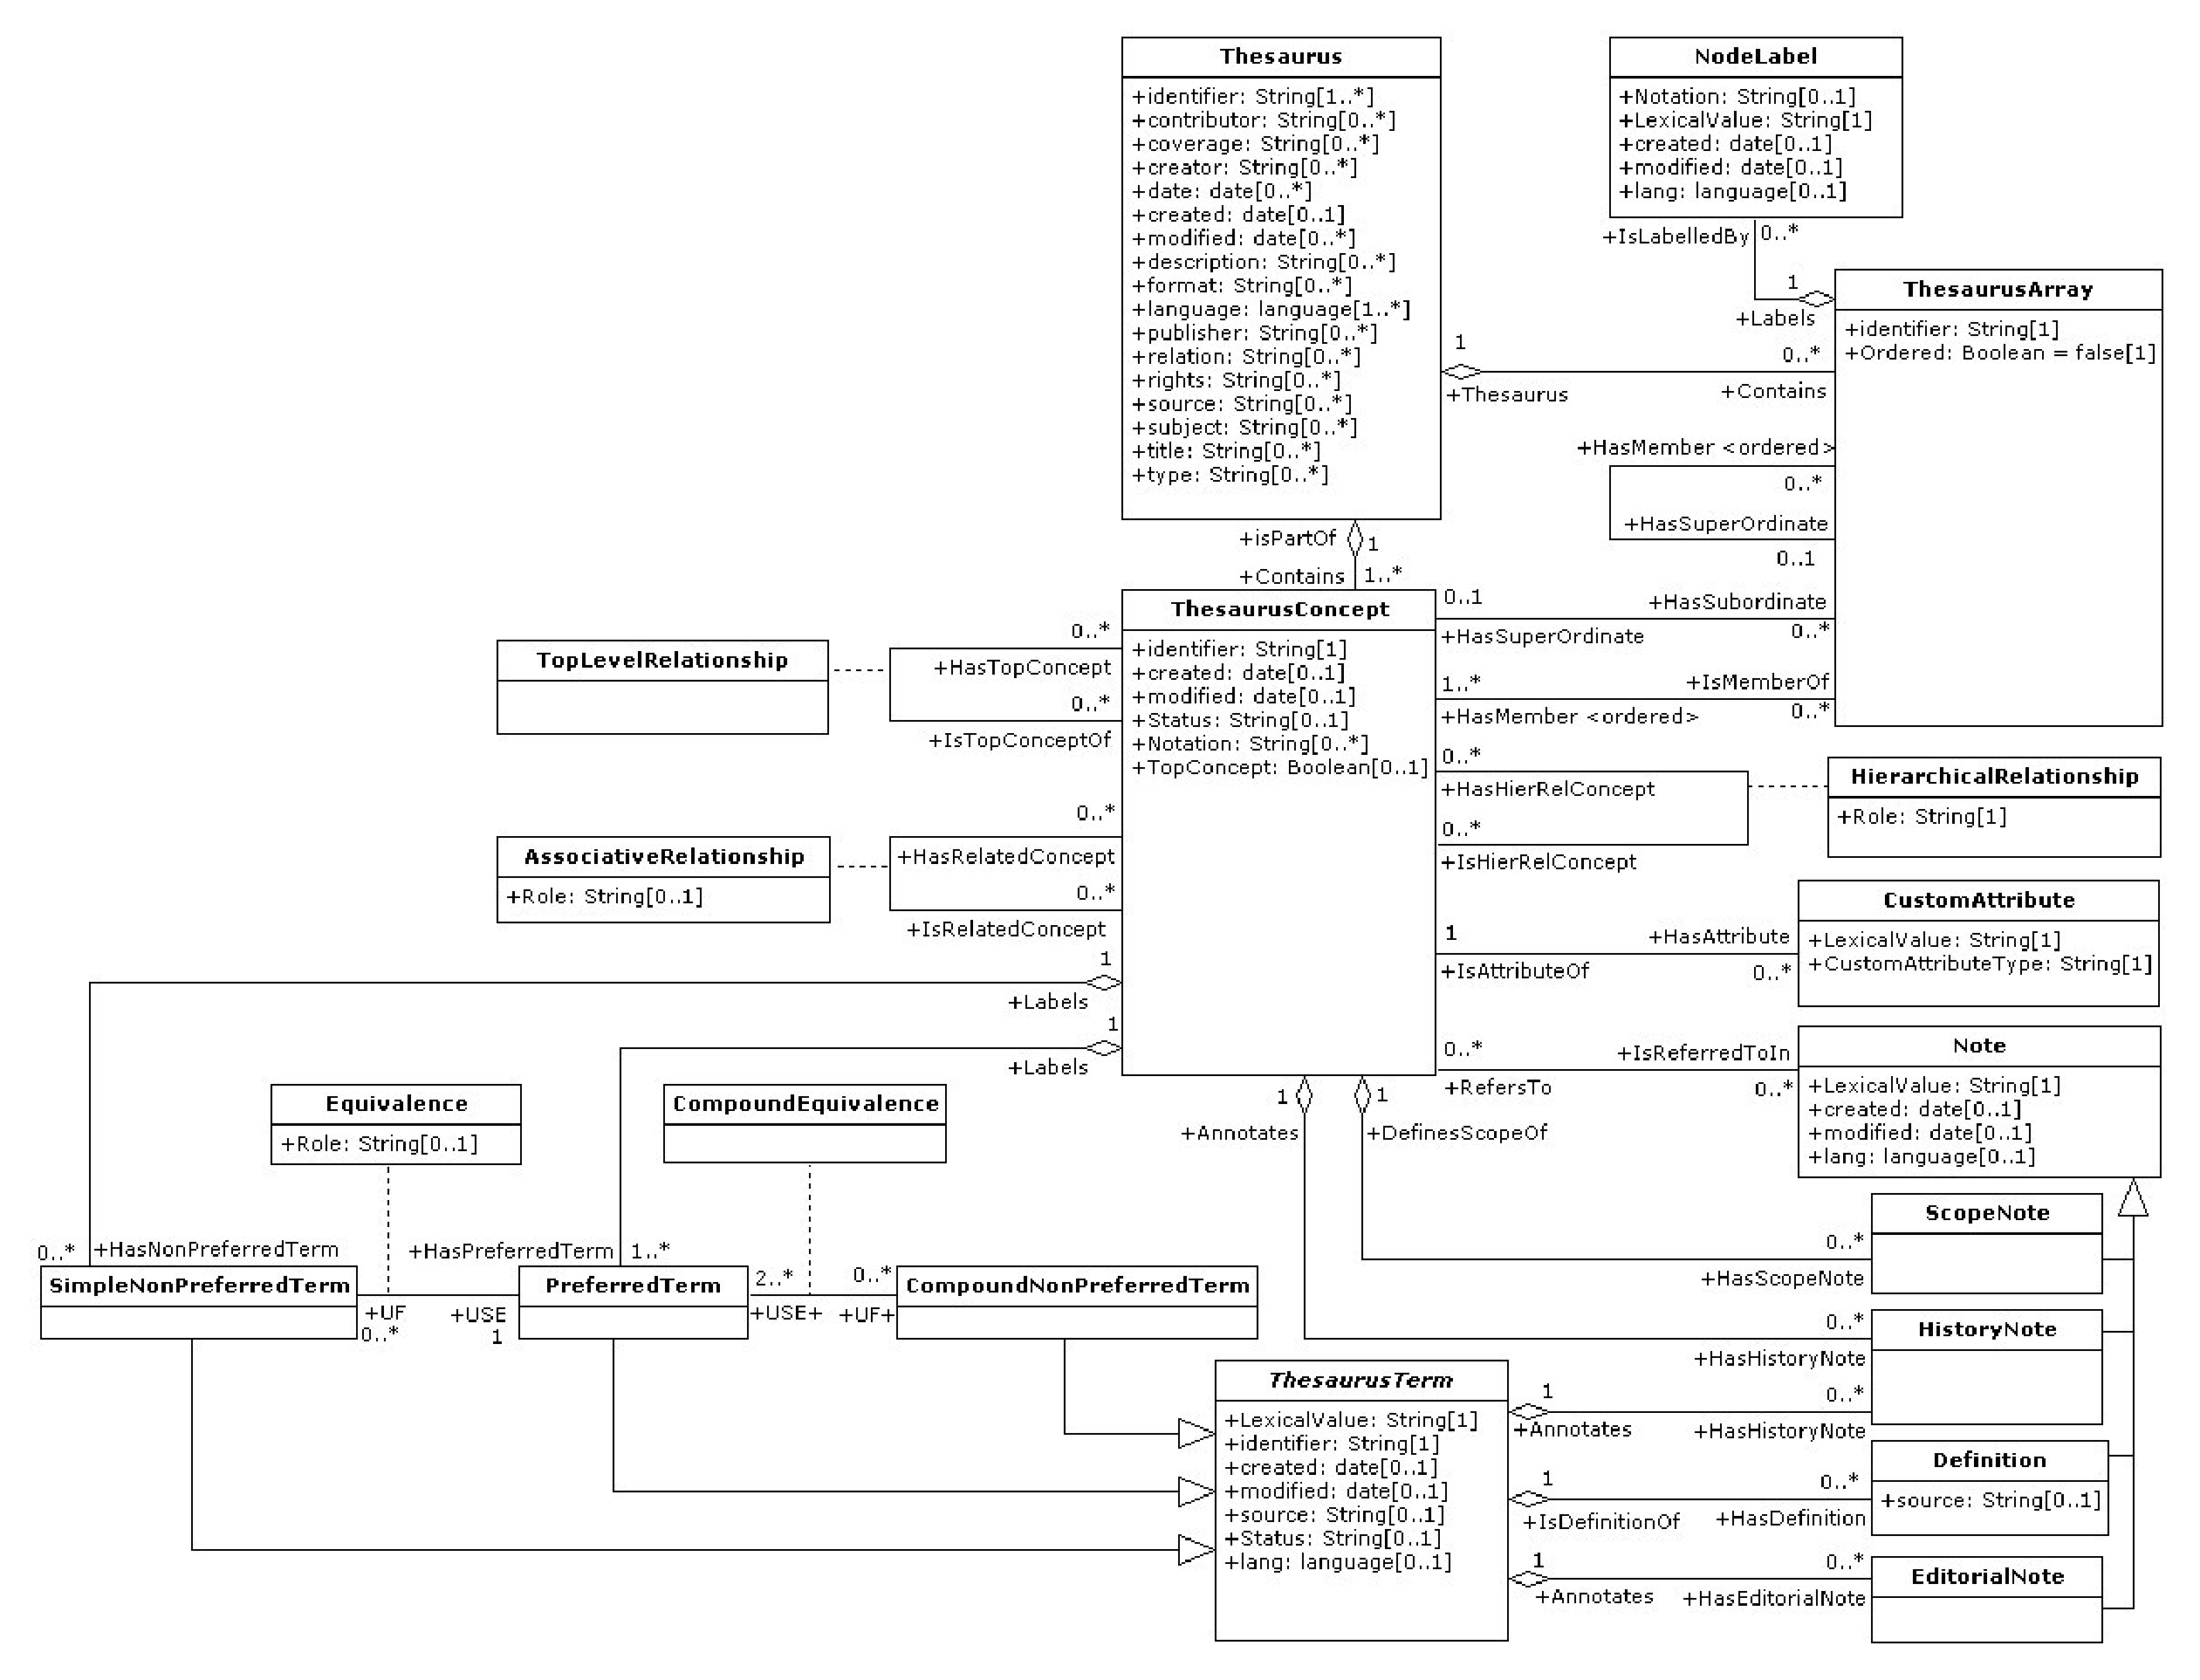
\includegraphics[width=13cm]{./Model.pdf}
\caption{Klasy wchodzące w skład tezaurusa, według normy BS8723}
\end{figure}


\section{Język SKOS}
\emph{Simple Knowledge Organization System} jest językiem, który pozwala na
tworzenie systemów organizacji wiedzy jak tezaurusy, schematy klasyfikacji,
systemy nagłówkowe oraz taksonomie. Modele, które są zapisane za pomocą SKOS,
mogą być łatwo przetwarzane przez maszyny, wymieniane pomiędzy aplikacjami
komputerowymi oraz publikowane w internecie.

Modele informacyjne utworzone w języku SKOS spełniają warunki 
\emph{OWL Full ontology} i mogą one zawierać również informacje zapisane za
pomocą OWL (\emph{Web Ontology Language}). SKOS podobnie jak OWL powstał w
oparciu o twierdzenia RDF (\emph{Resource Description Framework}) i formalna 
składnia jaką się posługuje to RDF/XML oraz Turtle \cite{SKOS-ref}. 

\subsubsection{Słownictwo}
Zasoby słownictwa jakim posługuje się SKOS znajdują się pod adresem:
\url{http://www.w3.org/2004/02/skos/core#}, w niniejszym dokumencie będzie on
opisany skrótem: \textbf{skos:}. Na podstawie \cite{SKOS-pr} dostępne są
następujące słowa kluczowe, które definiują klasy (słowa zaczynające się z
dużej litery) oraz właściwości (są pisane z małej litery):
\begin{itemize}
  \item \textbf{skos:Concept} - jednostka myśli, będąca abstrakcyjną encją
    niezależną od pojęć użytych do zetykietowania jej; semantyczna zawartość
    danego konceptu, może zostać wyrażona za pomocą kombinacji innych konceptów
    \cite{Willpower}:
  \item Etykiety - są cechami konceptów, które służą jako odnośniki do nich
    wyrażone w języku naturalnym. Skos pozwala na tworzynie etykiet w różnych
    językach w postaci:
\begin{verbatim}
"treść etykiety"@skrót_języka
\end{verbatim}
    Istnieją trzy rodzaje etykiet, które wzajemnie się wykluczają, więc nie
    dozwolone jest istnienie etykiet innego typu o tej samej treści
    \begin{itemize}
      \item \textbf{skos:prefLabel} - preferowana etykieta, może być tylko
        jedna dla danego konceptu; nie jest zabronione by różne koncepty
        zawierały tą samą etykietę, jednak zaleca się by takich przypadków
        nie było
      \item \textbf{skos:altLabel} - alternatywna etykieta, przydatna do
        określenia synonimów, jak również wyrazów bliskoznacznych oraz
        akronimów
      \item \textbf{skos:hiddenLabel} - ukryta etykieta, dostępnie jedynie
        wewnętrznie przez aplikację, w celu indeksowania i wyszukiwania, nie
        jest ona widoczna dla użytkownika; może służyć do uwzględniania
        literówek podczas poszukiwania danego konceptu
    \end{itemize}
  \item Relacje - służą do linkowania konceptów pomiędzy sobą, SKOS dostarcza
    następujące typy relacji:
    \begin{itemize}
      \item \textbf{skos:narrower} - hierarchiczne połączenie z konceptem
        bardziej szczegółowym na przykład:
\begin{verbatim}
ex:figuraGeometryczna rdf:type skos:Concept;
  skos:narrower ex:kwadrat.
ex:kwadrat rdf:type skos:Concept.
\end{verbatim}
      \item \textbf{skos:broader} - łączy z konceptem bardziej ogólnym:
\begin{verbatim}
ex:kwadrat rdf:type skos:Concept;
  skos:broader ex:figuraGeometryczna.
ex:figuraGeometryczna rdf:type skos:Concept.
\end{verbatim}
      \item \textbf{skos:related} - łączy z innym konceptem bez
        ustalania hierarchii, nie jest relacją tranzytywną
    \end{itemize}
    Pojęcia skos:broader i skos:narrower są przeciwieństwami, więc wystarczy
    określić tylko jedną z tych relacji, druga natomiast zostanie automatycznie
    przypisania w procesie wnioskowania OWL. Dodatkową cechą wyżej wymienionych
    relacji jest brak ich tranzytywności, czyli:
\begin{verbatim}
ex:figuraGeometryczna rdf:type skos:Concept;
  skos:narrower ex:prostokat.
ex:prostokat rdf:type skos:Concept;
  skos:narrower ex:kwadrat.
ex:kwadrat rdf:type skos:Concept.
\end{verbatim}
    nie implikuje relacji:
\begin{verbatim}
ex:figuraGeometryczna skos:narrower ex:kwadrat.
\end{verbatim}
    Jednak w \cite{SKOS-ref} opisane są tranzytywne wersje relacji
    \emph{broader} i \emph{narrower}: \textbf{skos:broaderTransitive},
    \textbf{skos:narrowerTransitive}, które umożliwiają z powyższej deklaracji
    wnioskować:
\begin{verbatim}
ex:figuraGeometryczna skos:narrowerTransitive ex:kwadrat.
\end{verbatim}
    Należy pamiętać również o tym, że poszczególne typy relacji wzajemnie się
    wykluczają.
  \item Przypisy dokumentacyjne - informacje w postaci zrozumiałej dla
    człowieka, przypisane do konceptu, w celu jego opisania:
    \begin{itemize}
      \item \textbf{skos:definition} - zawiera pełne wyjaśnienie znaczenia 
        danego konceptu
      \item \textbf{skos:example} - zawiera przykłady użycia konceptu
      \item \textbf{skos:scopeNote} - dostarcza częściowego znaczenia konceptu
        w szczególności określa zakres jego użycia
      \item \textbf{skos:historyNote} - opisuje znaczące zmiany jakie zaszły w 
        znaczeniu, bądź formie konceptu
      \item \textbf{skos:editorialNote} - informacja od autora, umieszczana 
        w celu ułatwienia utrzymania konceptu
      \item \textbf{skos:changeNote} - informacja o zmianach w koncepcie,
        umieszczona w celach administracyjnych
    \end{itemize}
  \item Schematy konceptów - służą do grupowania, pojedynczych konceptów, w
    celu ułatwienia indeksowania i tworzenia np. tezaurusów:
    \begin{itemize}
      \item \textbf{skos:ConceptScheme} - kontener będący schematem konceptów,
        zawierającym inne koncepty
      \item \textbf{skos:hasTopConcept} - przypisuje danemu schematowi,
        najwyższy w hierarchii koncept; może być kilka najwyższych konceptów
      \item \textbf{skos:topConceptOf} - przypisuje danemu konceptowi
        schemat konceptów, w którym będzie on najwyższy w hierarchii
      \item \textbf{skos:inScheme} - przypisuje danemu konceptowi schemat
        konceptów, w którym się znajduje, bez określenia hierarchii
    \end{itemize}
    Niestety w \cite{SKOS-ref} określone jest, że relacje pomiędzy konceptami
    (tzn. broader, narrower, itp.) nie są przenoszone na schemat konceptów,
    czyli:
\begin{verbatim}
ex:tezaurusAstronomiczny rdf:type skos:ConceptScheme;
  hasTopConcept ex:cialoNiebieskie.
ex:cialoNiebieskie rdf:type skos:Concept;
  skos:narrower ex:gwiazda.
ex:gwiazda rdf:type skos:Concept.
\end{verbatim}
    nie implikuje:
\begin{verbatim}
ex:gwiazda skos:inScheme ex:tezaurusAstronomiczny
\end{verbatim}
    \item Mapowanie konceptów pomiędzy schematami - SKOS dostarcza odpowiednich
      narzędzi, pozwalających mapować między sobą poszczególne koncepty w 
      różnych schematach:
      \begin{itemize}
        \item \textbf{skos:exactMatch} - dokładne dopasowanie, koncepty
          są identyczne
        \item \textbf{skos:closeMatch} - dopasowanie częściowe, które oznacza,
          że koncepty mogą być używane zamiennie, jednak w ograniczonym
          zakresie
        \item \textbf{skos:broaderMatch} - dopasowanie konceptu o bardziej
          ogólnym znaczeniu
        \item \textbf{skos:narrowerMatch} - dopasowanie konceptu o bardziej
          szczegółowym znaczeniu
        \item \textbf{skos:relatedMatch} - dopasowanie konceptu o powiązanym
          znaczeniu z danym konceptem bez wyróżnienia hierarchii
      \end{itemize}
    \item Kolekcje - służą do zgrupowania konceptów, które mogą zostać wspólnie
      dzielić tą samą etykietę:
      \begin{itemize}
        \item \textbf{skos:Collection} - kolekcja konceptów
        \item \textbf{skos:OrderedCollection} - kolekcja konceptów, których
          kolejność jest znacząca np w kolekcji ,,wykształcenie'' umieścić:
          \begin{enumerate}
            \item podstawowe
            \item średnie
            \item wyższe
          \end{enumerate}
        \item \textbf{skos:member} - przypisuje do danej kolekcji, wybrany
          koncept, użycie:
\begin{verbatim}
<kolekcja> skos:member <koncept>
\end{verbatim}
        \item \textbf{skos:memberList} - przypisuje do danej kolekcji, listę
          konceptów, użycie:
\begin{verbatim}
<kolekcja> skos:memberList (<koncept1> <koncept2>)
\end{verbatim}
      \end{itemize}
\end{itemize}
\bibliography{Literatura}
\addcontentsline{toc}{section}{Bibliografia}

\end{document}

\end{document}



\end{document}